%导演区
\documentclass[a4paper,11pt,UTF8]{article}%book,report,letter
\usepackage[table]{xcolor}
\usepackage{ctex}
\usepackage{geometry}
\geometry{a4paper,scale=0.8}
\usepackage{amsfonts}
\usepackage{amssymb}
\usepackage{verbatim}
\usepackage{mathrsfs}
\usepackage[arrow,matrix]{xy}
\usepackage{amsmath,amssymb,amscd,bm,bbm,amsthm,mathrsfs}
\usepackage{amsmath,amscd}
\usepackage{amsfonts,amssymb}
\usepackage{xypic}
\usepackage{indentfirst}
\usepackage{diagbox}
\usepackage{graphicx}
\usepackage{subfig}    %% 子图包
\usepackage{float} 
\usepackage{caption}
\captionsetup{labelfont=bf}
\usepackage{zhnumber} % change section number to chinese
%这下面为在latex中插入代码所需环境
\usepackage{CJK}
\usepackage{listings}
\usepackage{xcolor}
\lstset{
	language=Matlab,  %代码语言使用的是matlab
	frame=shadowbox, %把代码用带有阴影的框圈起来
	rulesepcolor=\color{red!20!green!20!blue!20},%代码块边框为淡青色
	keywordstyle=\color{blue!90}\bfseries, %代码关键字的颜色为蓝色,粗体
	commentstyle=\color{red!10!green!70}\textit,    % 设置代码注释的颜色
	showstringspaces=false,%不显示代码字符串中间的空格标记
	numbers=left, % 显示行号
	numberstyle=\tiny,    % 行号字体
	stringstyle=\ttfamily, % 代码字符串的特殊格式
	breaklines=true, %对过长的代码自动换行
	extendedchars=false,  %解决代码跨页时,章节标题,页眉等汉字不显示的问题
	texcl=true}
\def\d{\textup{d}}

\theoremstyle{plain}
\newtheorem{thm}{定理}[section]
\newtheorem{lem}{引理}[section]
\newtheorem{prop}{命题}[section]
\newtheorem{cor}{推论}[section]


\renewcommand{\qedsymbol}{$\square$}
\renewcommand\baselinestretch{1.25}
\renewcommand\thesection{\zhnum{section}}
\renewcommand \thesubsection {\arabic{section}}

\usepackage{tabu}                     % 表格插入
\usepackage{multirow}                 % 一般用以设计表格,将所行合并
\usepackage{multicol}                 % 合并多列
\usepackage{multirow}                % 合并多行
\usepackage{float}                    % 图片浮动
\usepackage{makecell}                 % 三线表-竖线
\usepackage{booktabs} 
%正文区
\begin{document}
	\title{\heiti 课题组组会-练习9}
	\author{王程 }
	\date{\today}
	\maketitle
	
	\section{练习及结果}
	1.对于$\varphi=\varphi\left(x,t\right)$考虑以下一维对流-扩散方程\\
	$$\left\{
	\begin{aligned}
		&\varphi_t+a\varphi_x=\nu\varphi_{xx}+f\left(x\right),x\in \left[0,1\right],t\geq 0.\\
		&\varphi\left(x,0\right)=x^2-x\\
		&\varphi\left(0,t\right)=\varphi\left(1,t\right)=0
	\end{aligned}
	\right.$$\\
	\indent 其中,$a=1,\nu=1,f\left(x\right)=\nu\pi^2sin\left(\pi x\right)+a\pi cos\left(\pi x\right)$。\\
	\indent 在均匀网格下,尝试在显式/隐式格式下使用Hyperbolic DG/rDG 的方法求上述方程的稳态解,并与解析解进行比较,空间离散方式可选用DG(P0P1)+DG(P0),DG(P0P2)+rDG(P0P1),DG(P0P2)+DG(P1)。\\
	\indent 调整系数$a,\nu$,在不同的雷诺数下进行比较数值解和解析解。\\
	~\\
	\indent 2.考虑非稳态的一维对流-扩散方程,其中精确解为
	$$\varphi\left(x,t\right)=\frac{1}{\sqrt{4t+1}}exp\left(-\frac{\left(x-at-x_0\right)^2}{\nu \left(4t+1\right)}\right),0\leq x\leq 2.$$\\
	\indent 其中,$a=10^4,\nu=0.01,x_0=0.5.$\\
	物理时间步长设置为$10^{-9}$,在均匀网格$\left(Nelem=32,64,128,256\right)$下,尝试在双时间步法下使用Hyperbolic DG/rDG的方法求上述方程在t=$10^{-6}$时刻的数值解,并与解析解进行比较。\\
	\clearpage
	\noindent \textbf{解:1.}\\
	\indent 
	a).为对比Explicit与Implicit方法的不同,考虑在不同空间离散格式下固定雷诺数为1:$a=1,\nu=1$,对比Explicit与Implicit方法的数值解:\\
	\begin{table}[H]
		\centering
		\caption{DG(P0P1)+DG(P0) Explicit 与 Implicit数值解对比}
		\label{tbl:table1}
		\begin{tabular}{cccccc}
			\Xhline{2pt}
			\multicolumn{2}{c}{$Re=\frac{|a|}{\nu}=1:a=1,\nu=1$}\\
						\Xhline{0.5pt}\\
			\multicolumn{2}{c}{Nelement}& 8& 16& 32& 64 \\
						\Xhline{0.5pt}\\
 
			\multicolumn{2}{c}{Explicit} $CFL_\tau=0.01,tol=10^{-8}$\\

			
%			\multirow{2}{*}{Num of cells} & \multicolumn{2}{c}{P1P2(LSR)} & \multicolumn{2}{c}{P1P2(LSr)} & \multicolumn{2}{c}{P1P2(HLSr)}  \\
%			\Xcline{2-3}{0.4pt} 	\Xcline{4-5}{0.4pt} 	\Xcline{6-7}{0.4pt}
%			& L2-errors& order &L2-errors& order &L2-errors& order\\
		    \Xcline{1-2}{0.4pt}\\
			\multicolumn{2}{c}{$L_2errors-{U}$}& 0.0629& 0.0327& 0.0167& 0.0084\\
			\multicolumn{2}{c}{$L_2errors-{U_x}$}& 0.2563& 0.1272& 0.0634& 0.0317\\			
			\multicolumn{2}{c}{$Matlab$运行时间(s)}& 1.2203& 1.774& 4.404& 12.701\\
			\\
			\multicolumn{2}{c}{Implicit} $CFL_\tau=100,tol=10^{-8}$\\
		    \Xcline{1-2}{0.4pt}\\
			\multicolumn{2}{c}{$L_2errors-{U}$}& 0.0540& 0.0321& 0.0167& 0.0084\\
			\multicolumn{2}{c}{$L_2errors-{U_x}$}& 0.2625& 0.1274& 0.0634& 0.0317\\			
			\multicolumn{2}{c}{$Matlab$运行时间(s)}& 0.762& 0.909& 0.812& 0.890\\

			\Xhline{2pt}
		\end{tabular} 
	\end{table}


	\begin{table}[H]
	\centering
	\caption{DG(P0P2)+DG(P1) Explicit 与 Implicit数值解对比}
	\label{tbl:table2}
	\begin{tabular}{cccccc}
		\Xhline{2pt}
		\multicolumn{2}{c}{$Re=\frac{|a|}{\nu}=1:a=1,\nu=1$}\\
		\Xhline{0.5pt}\\
		\multicolumn{2}{c}{Nelement}& 8& 16& 32& 64 \\
		\Xhline{0.5pt}\\
		
		\multicolumn{2}{c}{Explicit} $CFL_\tau=0.01,tol=10^{-8}$\\
		
		
		%			\multirow{2}{*}{Num of cells} & \multicolumn{2}{c}{P1P2(LSR)} & \multicolumn{2}{c}{P1P2(LSr)} & \multicolumn{2}{c}{P1P2(HLSr)}  \\
		%			\Xcline{2-3}{0.4pt} 	\Xcline{4-5}{0.4pt} 	\Xcline{6-7}{0.4pt}
		%			& L2-errors& order &L2-errors& order &L2-errors& order\\
		\Xcline{1-2}{0.4pt}\\
		\multicolumn{2}{c}{$L_2errors-{U}$}& 0.0092& 0.0023& $5.83\times 10^{-4}$& $1.60\times 10^{-4}$\\
		\multicolumn{2}{c}{$L_2errors-{U_x}$}& 0.0311& 0.0078& 0.0020& $5.86\times 10^{-4}$\\			
		\multicolumn{2}{c}{$Matlab$运行时间(s)}& 1.116& 1.388& 2.959& 8.147\\
		\\
		\multicolumn{2}{c}{Implicit} $CFL_\tau=100,tol=10^{-8}$\\
		\Xcline{1-2}{0.4pt}\\
		\multicolumn{2}{c}{$L_2errors-{U}$}& 0.0188& 0.0031& $5.92\times 10^{-4}$& $1.43\times 10^{-4}$\\
		\multicolumn{2}{c}{$L_2errors-{U_x}$}& 0.0602& 0.0101& 0.002& $4.85\times 10^{-4}$\\			
		\multicolumn{2}{c}{$Matlab$运行时间(s)}& 0.774& 0.918& 0.970& 1.086\\
		
		\Xhline{2pt}
	\end{tabular} 
\end{table}

	\begin{table}[H]
	\centering
	\caption{DG(P0P2)+rDG(P0P1) Explicit 与 Implicit数值解对比}
	\label{tbl:table3}
	\begin{tabular}{cccccc}
		\Xhline{2pt}
		\multicolumn{2}{c}{$Re=\frac{|a|}{\nu}=1:a=1,\nu=1$}&\multicolumn{4}{c}{$\omega_0=1,\omega_1=1,\omega_2=1,\omega_b=0$}\\
		\Xhline{0.5pt}\\
		\multicolumn{2}{c}{Nelement}& 8& 16& 32& 64 \\
		\Xhline{0.5pt}\\
		
		\multicolumn{2}{c}{Explicit} $CFL_\tau=0.01,tol=10^{-8}$\\
		
		
		%			\multirow{2}{*}{Num of cells} & \multicolumn{2}{c}{P1P2(LSR)} & \multicolumn{2}{c}{P1P2(LSr)} & \multicolumn{2}{c}{P1P2(HLSr)}  \\
		%			\Xcline{2-3}{0.4pt} 	\Xcline{4-5}{0.4pt} 	\Xcline{6-7}{0.4pt}
		%			& L2-errors& order &L2-errors& order &L2-errors& order\\
		\Xcline{1-2}{0.4pt}\\
		\multicolumn{2}{c}{$L_2errors-{U}$}& 0.0315& 0.0106& 0.0026& $6.32\times 10^{-4}$\\
		\multicolumn{2}{c}{$L_2errors-{U_x}$}&0.0694& 0.0148& 0.003& $6.95\times 10^{-4}$\\			
		\multicolumn{2}{c}{$Matlab$运行时间(s)}& 0.978& 1.635& 3.209& 9.406\\
		\\
		\multicolumn{2}{c}{Implicit} $CFL_\tau=100,tol=10^{-8}$\\
		\Xcline{1-2}{0.4pt}\\
		\multicolumn{2}{c}{$L_2errors-{U}$}& 0.0414& 0.0111& 0.0026& $6.16\times 10^{-4}$\\
		\multicolumn{2}{c}{$L_2errors-{U_x}$}& 0.0747&0.0157& 0.003& $6.10\times 10^{-4}$\\			
		\multicolumn{2}{c}{$Matlab$运行时间(s)}& 0.748& 0.771& 0.806& 0.95\\
		
		\Xhline{2pt}
	\end{tabular} 
\end{table}\leavevmode\\
\indent 观察表1,表2和表3,可以发现Explicit与Implicit最主要的区别是运行时间,两者的$L_2errors$差别不大。\\
~\\
	\indent 
b).调整系数$a,\nu$,考虑雷诺数为0,1,2,10,20时数值解与解析解的$L_2$误差,绘制成下图(仅展示Implicit,Nelem=8,64的情况):
	\begin{figure}[H]
	\centering
	\subfloat[U(Nelem=8)]{
		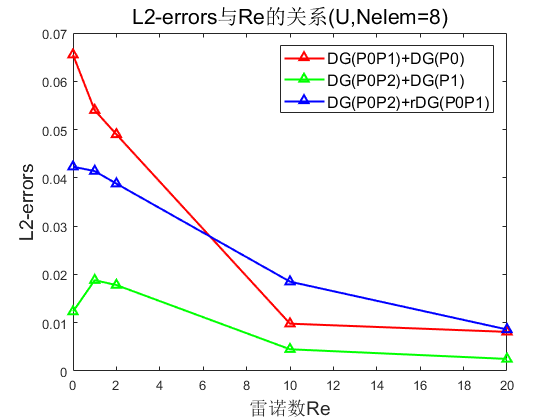
\includegraphics[width=3in]{Stable-problem/Advection-Diffusion-Eq-Implicit/L2errors-Re-U8.png} 
	}
	\hfill
	\subfloat[U(Nelem=64)]{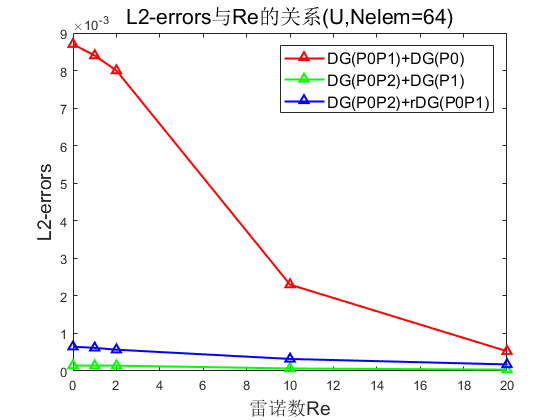
\includegraphics[width=3in]{Stable-problem/Advection-Diffusion-Eq-Implicit/L2errors-Re-U64.png} }
	\caption{$L_2errors-U$和Re的关系}
\end{figure}\leavevmode\\
	\begin{figure}[H]
	\centering
		\subfloat[Ux(Nelem=8)]{
		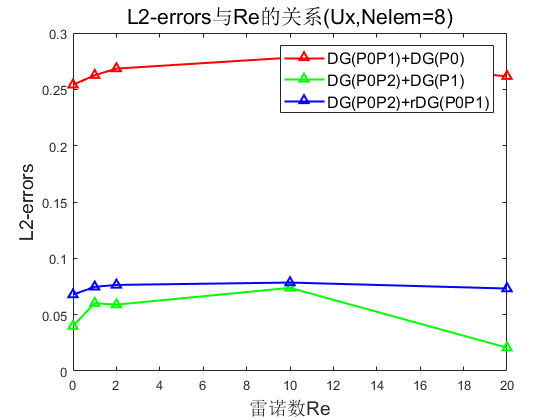
\includegraphics[width=3in]{Stable-problem/Advection-Diffusion-Eq-Implicit/L2errors-Re-Ux8.png} 
	}
	\hfill
	\subfloat[Ux(Nelem=64)]{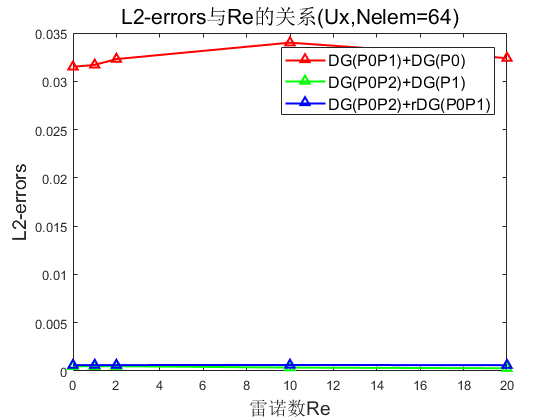
\includegraphics[width=3in]{Stable-problem/Advection-Diffusion-Eq-Implicit/L2errors-Re-Ux64.png} }
	\caption{$L_2errors-U_x$和Re的关系}
\end{figure}\leavevmode\\
\indent 观察图1和图2,可以很明显的发现$L_2errors-U$会随着雷诺数Re的增大而减小,而$L_2errors-U_x$对雷诺数的变化并不敏感。\\

\noindent \textbf{解:2.}\\
\indent 对于非稳态的一维对流-扩散方程,由于其精确解为:	
$$\varphi\left(x,t\right)=\frac{1}{\sqrt{4t+1}}exp\left(-\frac{\left(x-at-x_0\right)^2}{\nu \left(4t+1\right)}\right),0\leq x\leq 2.$$\\
当t$\rightarrow$$\infty$时,$\varphi$$\rightarrow$ 0.因此,实际考虑的方程为\\
	$$\left\{
\begin{aligned}
	&\varphi_t+a\varphi_x=\nu\varphi_{xx},x\in \left[0,2\right],t\geq 0.\\
	&\varphi\left(x,0\right)=exp\left(-\frac{\left(x-x_0\right)^2}{\nu}\right)\\
	&\varphi\left(0,t\right)=\varphi\left(1,t\right)=0
\end{aligned}
\right.$$\\
\indent 仅考虑Implicit,对该方程进行求解,得到如下表格:\\
	\begin{table}[H]
	\centering
	\caption{Implicit数值解与解析解对比}
	\label{tbl:table4}
	\begin{tabular}{cccccc}
		\Xhline{2pt}
		\multicolumn{2}{c}{$Re=\frac{|a|}{\nu}=10^6:a=10^4,\nu=0.01,x_0=0.5$}&\multicolumn{4}{c}{$CFL_\tau=10^6,tol=10^{-5}$}\\
		\Xhline{0.5pt}\\
		\multicolumn{2}{c}{Nelement(Implicit)}& 32& 64& 128& 256 \\
		\Xhline{0.5pt}\\
		
		\multicolumn{2}{c}{DG(P0P1)+DG(P0)} \\
		
		
		%			\multirow{2}{*}{Num of cells} & \multicolumn{2}{c}{P1P2(LSR)} & \multicolumn{2}{c}{P1P2(LSr)} & \multicolumn{2}{c}{P1P2(HLSr)}  \\
		%			\Xcline{2-3}{0.4pt} 	\Xcline{4-5}{0.4pt} 	\Xcline{6-7}{0.4pt}
		%			& L2-errors& order &L2-errors& order &L2-errors& order\\
		\Xcline{1-2}{0.4pt}\\
		\multicolumn{2}{c}{$L_2errors-{U}$}& 0.8834& 0.8830& 0.8830& 0.8830\\
		\multicolumn{2}{c}{$L_2errors-{U_x}$}&4.5617& 4.3956& 4.3668& 4.3601\\			
		\multicolumn{2}{c}{$Matlab$运行时间(s)}& 5.942& 10.444& 20.205& 46.048\\
		\\
		\multicolumn{2}{c}{DG(P0P2)+DG(P1)}\\
		\Xcline{1-2}{0.4pt}\\
		\multicolumn{2}{c}{$L_2errors-{U}$}& 0.8833& 0.8832&0.8830& 0.8830\\
		\multicolumn{2}{c}{$L_2errors-{U_x}$}& 4.4851&4.4337& 4.3795& 4.3629\\			
		\multicolumn{2}{c}{$Matlab$运行时间(s)}&6.287& 20.087& 84.785& 429.929\\
		\\
		\multicolumn{2}{c}{DG(P0P2)+rDG(P0P1)}&\multicolumn{4}{c}{$\omega_0=1,\omega_1=1,\omega_2=1,\omega_b=0$}\\
        \Xhline{0.4pt}\\
        \multicolumn{2}{c}{$L_2errors-{U}$}& 0.8832& 0.8830& 0.8830& 0.8830\\
        \multicolumn{2}{c}{$L_2errors-{U_x}$}& 4.4539&4.3620& 4.3578& 4.3578\\			
        \multicolumn{2}{c}{$Matlab$运行时间(s)}&5.896& 13.474& 21.430& 35.701\\		
		
		\Xhline{2pt}
	\end{tabular} 
\end{table}\leavevmode\\
\indent \textbf{观察表4,可以发现:}\\
~\\
\indent 1).在非稳态问题中,CFL足够大时,隐式格式所需要的时间也不短(部分原因是Matlab处理循环较慢),这也侧面凸显出相较于显示格式,隐式格式在缩短运行时间方面有着巨大优势。\\
\indent 2).rDG的优点。\\
\indent 3).上述三种空间离散格式,当Nelem达到32即以上,$L_2errors-U$和$L_2errors-U_x$不随网格的加密而减小。\\
~\\
\indent 下面展示上述三种空间离散格式下的数值解与解析解比较图(Nelem=32):\\
\clearpage
\textbf{DG(P0P1)+DG(P0)}
	\begin{figure}[H]
	\centering
	\subfloat[U(Nelem=32)]{
		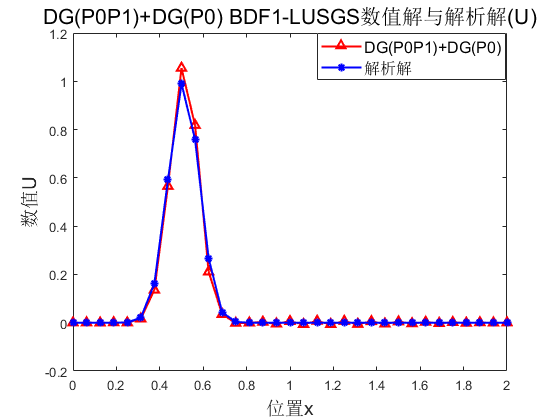
\includegraphics[width=3in]{Nonstable-problem/Advection-Diffusion-Eq-Implicit/DGP0P1plusDGP0/U32.png} 
	}
	\hfill
	\subfloat[Ux(Nelem=32)]{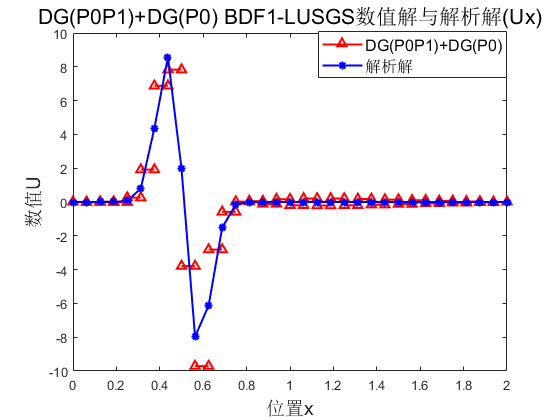
\includegraphics[width=3in]{Nonstable-problem/Advection-Diffusion-Eq-Implicit/DGP0P1plusDGP0/Ux32.png} }
	\caption{DG(P0P1)+DG(P0)数值解与解析解比较图}
\end{figure}\leavevmode\\
~\\
\textbf{DG(P0P2)+DG(P1)}
\begin{figure}[H]
	\centering
	\subfloat[U(Nelem=32)]{
		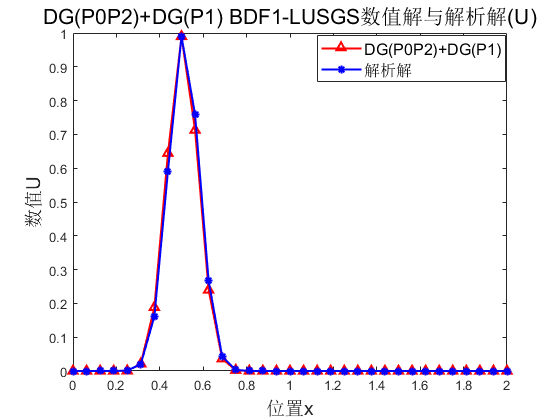
\includegraphics[width=3in]{Nonstable-problem/Advection-Diffusion-Eq-Implicit/DGP0P2plusDGP1/U32.png} 
	}
	\hfill
	\subfloat[Ux(Nelem=32)]{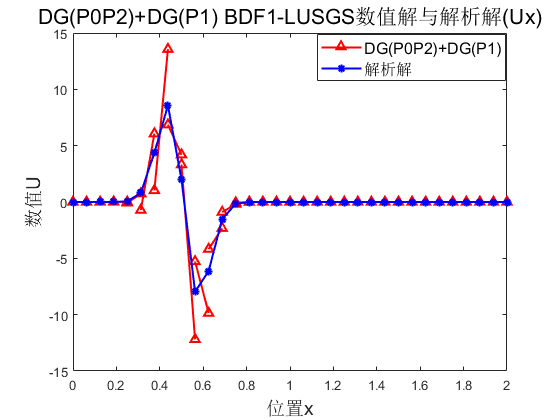
\includegraphics[width=3in]{Nonstable-problem/Advection-Diffusion-Eq-Implicit/DGP0P2plusDGP1/Ux32.png} }
	\caption{DG(P0P2)+DG(P1)数值解与解析解比较图}
\end{figure}\leavevmode
\clearpage
\textbf{DG(P0P2)+rDG(P0P1)}
\begin{figure}[H]
	\centering
	\subfloat[U(Nelem=32)]{
		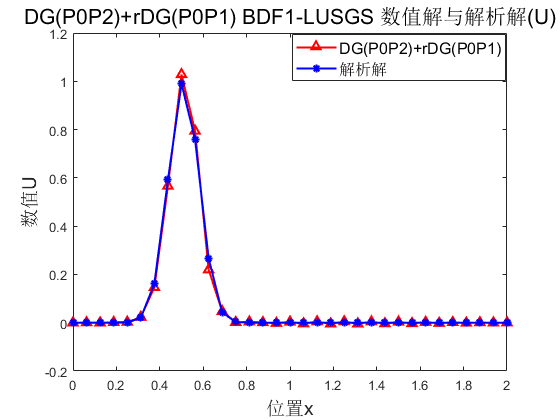
\includegraphics[width=3in]{Nonstable-problem/Advection-Diffusion-Eq-Implicit/DGP0P2plusrDGP0P1/U32.png} 
	}
	\hfill
	\subfloat[Ux(Nelem=32)]{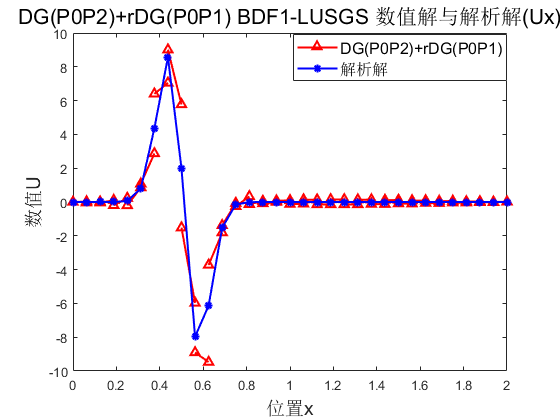
\includegraphics[width=3in]{Nonstable-problem/Advection-Diffusion-Eq-Implicit/DGP0P2plusrDGP0P1/Ux32.png} }
	\caption{DG(P0P2)+rDG(P0P1)数值解与解析解比较图}
\end{figure}\leavevmode\\
\clearpage
\section{附录}
\subsubsection{代码(仅展示部分,详细见Github)}
\noindent \textbf{Nonstable-problem-Advection-Diffusion-Eq-Implicit-DGP0P1plusDGP0}
\lstset{language=Matlab}%代码语言使用的是matlab
\lstset{breaklines}%自动将长的代码行换行排版
\lstset{extendedchars=false}%解决代码跨页时,章节标题,页眉等汉字不显示的问题
\begin{lstlisting}
clc
clear all
close all
% Preproceeding
%Some basic paramater
Unit=32;%单元个数
nu=0.01;a=10^4;x0=0.5;
Lr=1/max(2*pi,abs(a)/nu);Tr=Lr^2/nu;abslambda=sqrt(nu/Tr);A1=[abslambda+abs(a),0;0,abslambda];A=[a,-nu;-1/Tr,0];B1=1;
deltat=10^(-9);
CFLtau=10^6;
endtau=10;%伪时间阈值
endt=10^(-6);
tol=10^(-5);%跳出循环条件
belta=0;%网格扰动系数
endx=2;deltax=endx/Unit;numberx=endx/deltax+1;
Vcurrent=zeros(2,numberx-1);
Vn=zeros(2,numberx-1);
Vm=zeros(2,numberx-1);
Vm1=zeros(2,numberx-1);
dimention=2;
%LHS
LHS1=zeros(dimention*Unit,dimention*Unit);
LHS2=zeros(dimention*Unit,dimention*Unit);
LHS3=zeros(dimention*Unit,dimention*Unit);
%RHS
R=zeros(dimention*Unit,1);
Rd=zeros(dimention*Unit,1);
Rb=zeros(dimention*Unit,1);
Fn=zeros(2,numberx);
%记录内点位置,上下浮动不超过belta
Grid=zeros(1,numberx);
Deltax=zeros(1,Unit);
for i=2:numberx-1
Grid(1,i)=(i-1)*deltax+(2*rand(1)-1)*belta*deltax;
end
Grid(1,numberx)=endx;
%记录每个单元的区间长度
for i=2:numberx
Deltax(i-1)=Grid(1,i)-Grid(1,i-1);
end

%伪时间上的local time stepping
deltatau=zeros(1,numberx-1);%伪时间变量
for i=1:numberx-1
deltatau(i)=CFLtau*(Grid(1,i+1)-Grid(1,i))/(abslambda+abs(a));%伪时间变量
end

%计算order
Acc=zeros(3,4);a1=[1/(2*32),1/(2*64),1/(2*128),1/(2*256)];a2=[1/(2*32),1/(2*64)];
%记录每个物理时间步上的伪时间终止时刻
n=zeros(1,floor(endt/deltat));
%solve the exasolution
Uexasolution=zeros(2,numberx); Vnumsolution=zeros(2,numberx-1);
for k=1:numberx
Uexasolution(1,k)=1/sqrt(4*endt+1)*exp(-(Grid(k)-a*endt-x0)^2/(nu*(4*endt+1)));
Uexasolution(2,k)=1/sqrt(4*endt+1)*exp(-(Grid(k)-a*endt-x0)^2/(nu*(4*endt+1)))*(-2*(Grid(k)-a*endt-x0)/(nu*(4*endt+1)));
end

%% Proceeding

%构建LHS
%Mtau/deltatau
for i=1:Unit
LHS1(dimention*(i-1)+1,dimention*(i-1)+1)=Deltax(i)/deltatau(i);
LHS1(dimention*(i-1)+2,dimention*(i-1)+2)=(Deltax(i)/12+1/Deltax(i))/deltatau(i);
end
%Rdomain
for i=1:Unit
LHS2(dimention*(i-1)+2,dimention*(i-1)+2)=(1/Tr+nu)/Deltax(i);
LHS2(dimention*(i-1)+2,dimention*(i-1)+1)=-a;
end

%Rboundary
for iface=2:numberx-1
ieL=iface-1;
ieR=iface;
CL=[B1,1/2;0,B1/Deltax(ieL)];
CR=[B1,-1/2;0,B1/Deltax(ieR)];
%diag
LHS3(dimention*(ieL-1)+1:dimention*ieL,dimention*(ieL-1)+1:dimention*ieL)=LHS3(dimention*(ieL-1)+1:dimention*ieL,dimention*(ieL-1)+1:dimention*ieL)+0.5*CL'*(A+A1)*CL;
LHS3(dimention*(ieR-1)+1:dimention*ieR,dimention*(ieR-1)+1:dimention*ieR)=LHS3(dimention*(ieR-1)+1:dimention*ieR,dimention*(ieR-1)+1:dimention*ieR)-0.5*CR'*(A-A1)*CR;
%upper
LHS3(dimention*(ieL-1)+1:dimention*ieL,dimention*(ieR-1)+1:dimention*ieR)=LHS3(dimention*(ieL-1)+1:dimention*ieL,dimention*(ieR-1)+1:dimention*ieR)+0.5*CL'*(A-A1)*CR;
%lower
LHS3(dimention*(ieR-1)+1:dimention*ieR,dimention*(ieL-1)+1:dimention*ieL)=LHS3(dimention*(ieR-1)+1:dimention*ieR,dimention*(ieL-1)+1:dimention*ieL)-0.5*CR'*(A+A1)*CL;
end

%边界:左
iface=1;
ieR=iface;
CR=[B1,-1/2;0,B1/Deltax(ieR)];
LHS3(dimention*(ieR-1)+1:dimention*ieR,dimention*(ieR-1)+1:dimention*ieR)=LHS3(dimention*(ieR-1)+1:dimention*ieR,dimention*(ieR-1)+1:dimention*ieR)-CR'*(0.5*(A+A1)*[0,0;0,1]*CR+0.5*(A-A1)*CR);
%边界:右
iface=numberx;
ieL=iface-1;
CL=[B1,1/2;0,B1/Deltax(ieL)];
LHS3(dimention*(ieL-1)+1:dimention*ieL,dimention*(ieL-1)+1:dimention*ieL)=LHS3(dimention*(ieL-1)+1:dimention*ieL,dimention*(ieL-1)+1:dimention*ieL)+CL'*(0.5*(A+A1)+0.5*(A-A1)*[0,0;0,1])*CL;

%组装LHS
LHS=LHS1+LHS2+LHS3;

%Mt/deltat
for i=1:Unit
LHS(dimention*(i-1)+1,dimention*(i-1)+1)=LHS(dimention*(i-1)+1,dimention*(i-1)+1)+Deltax(i)/deltat;
LHS(dimention*(i-1)+2,dimention*(i-1)+2)=LHS(dimention*(i-1)+2,dimention*(i-1)+2)+(Deltax(i)/12)/deltat;
end


%initial  condition set up
for k=1:numberx-1
%利用Gauss积分计算Vcurrent
t=[-sqrt(15)/5,0,sqrt(15)/5];
W=[5/9,8/9,5/9];
xci=(Grid(k+1)+Grid(k))/2;
for ig=1:3
xig=Deltax(k)/2*t(ig)+xci;
const=W(ig)*0.5*Deltax(k);
Vcurrent(1,k)=Vcurrent(1,k)+const*exp(-(xig-x0)^2/nu);
Vcurrent(2,k)=Vcurrent(2,k)+const*exp(-(xig-x0)^2/nu)*(-2*(xig-x0)/nu);
end 
Vcurrent(1,k)=Vcurrent(1,k)/Deltax(k);


end
%对t=0时刻赋值
Vn=Vcurrent;
i=1;
for itime=0:deltat:endt
Vm=Vn;
for itau=0:min(deltatau):endtau
%组装RHS
%利用Gauss积分计算Rdomain
t=[-sqrt(15)/5,0,sqrt(15)/5];
W=[5/9,8/9,5/9];
for ie=1:Unit
xci=(Grid(ie+1)+Grid(ie))/2;
for ig=1:3
xig=Deltax(ie)/2*t(ig)+xci;
B2g=(xig-xci)/Deltax(ie);
varphig=Vm(1,ie)+B2g*Vm(2,ie);
Vg=Vm(2,ie)/Deltax(ie);
S1g=0;
S2g=-Vg/Tr;
F1g=a*varphig-nu*Vg;
F2g=-varphig/Tr;
const=W(ig)*0.5*Deltax(ie);
Rd(2*(ie-1)+1)=Rd(2*(ie-1)+1)+S1g*const;
Rd(2*(ie-1)+2)=Rd(2*(ie-1)+2)+(S1g*B2g+S2g/Deltax(ie)+F1g/Deltax(ie))*const;


end
end



%Rboundary
for iface=2:numberx-1
ieL=iface-1;
ieR=iface;
B2L=1/2;
B2R=-1/2;
varphiL=Vm(1,ieL)+B2L*Vm(2,ieL);
varphiR=Vm(1,ieR)+B2R*Vm(2,ieR);
VL=Vm(2,ieL)/Deltax(ieL);
VR=Vm(2,ieR)/Deltax(ieR);

Fn(:,iface)=0.5*([a*varphiL-nu*VL;-varphiL/Tr]+[a*varphiR-nu*VR;-varphiR/Tr])-0.5*A1*([varphiR;VR]-[varphiL;VL]);
Rb(2*(ieL-1)+1)=Rb(2*(ieL-1)+1)-Fn(1,iface);
Rb(2*(ieL-1)+2)=Rb(2*(ieL-1)+2)-Fn(1,iface)*B2L-Fn(2,iface)/Deltax(ieL);
%     Rb(dimention*(ieL-1)+3)=Rb(dimention*(ieL-1)+3)-Fn(1,iface)*B3L-Fn(2,iface)*B2L/Deltax(ieL);
Rb(2*(ieR-1)+1)=Rb(2*(ieR-1)+1)+Fn(1,iface);
Rb(2*(ieR-1)+2)=Rb(2*(ieR-1)+2)+Fn(1,iface)*B2R+Fn(2,iface)/Deltax(ieR);
%     Rb(dimention*(ieR-1)+3)=Rb(dimention*(ieR-1)+3)+Fn(1,iface)*B3R+Fn(2,iface)*B2R/Deltax(ieR);
end
%边界:左
iface=1;
ieR=iface;
B2R=-1/2;
varphiR=Vm(1,ieR)+B2R*Vm(2,ieR);
VR=Vm(2,ieR)/Deltax(ieR);
Fn(:,iface)=0.5*([-nu*VR;0]+[a*varphiR-nu*VR;-varphiR/Tr])-0.5*A1*([varphiR;VR]-[0;VR]);
Rb(2*(ieR-1)+1)=Rb(2*(ieR-1)+1)+Fn(1,iface);
Rb(2*(ieR-1)+2)=Rb(2*(ieR-1)+2)+Fn(1,iface)*B2R+Fn(2,iface)/Deltax(ieR);
% Rb(dimention*(ieR-1)+3)=Rb(dimention*(ieR-1)+3)+Fn(1,iface)*B3R+Fn(2,iface)*B2R/Deltax(ieR);

%边界:右
iface=numberx;
ieL=iface-1;
B2L=1/2;
varphiL=Vm(1,ieL)+B2L*Vm(2,ieL);
VL=Vm(2,ieL)/Deltax(ieL);
Fn(:,iface)=0.5*([a*varphiL-nu*VL;-varphiL/Tr]+[-nu*VL;0])-0.5*A1*([0;VL]-[varphiL;VL]);
Rb(2*(ieL-1)+1)=Rb(2*(ieL-1)+1)-Fn(1,iface);
Rb(2*(ieL-1)+2)=Rb(2*(ieL-1)+2)-Fn(1,iface)*B2L-Fn(2,iface)/Deltax(ieL);
% Rb(dimention*(ieL-1)+3)=Rb(dimention*(ieL-1)+3)-Fn(1,iface)*B3L-Fn(2,iface)*B2L/Deltax(ieL);

%R组装
R=Rd+Rb;

for k=1:Unit
Mt=[Deltax(k),0;0,Deltax(k)/12];
R(2*k-1:2*k,1)=R(2*k-1:2*k,1)-Mt*(Vm(:,k)-Vn(:,k))/deltat;
end

X=LUSGS(LHS,R,Unit);
if max(abs(X))<tol&&itau>=min(deltatau)
break;
end
for k=1:Unit
Vm1(:,k)=Vm(:,k)+X(2*k-1:2*k,1);
end

Vm=Vm1;
Rd=zeros(dimention*Unit,1);
Rb=zeros(dimention*Unit,1);

end
n(i)=itau;i=i+1;    
Vn=Vm1;    
end

Vnumsolution=Vn;

%% Post-proceeding
%U
figure
k=1;
x=Grid(k):1*(Grid(k+1)-Grid(k)):Grid(k+1);
xci=(Grid(k+1)+Grid(k))/2;
p=@(x)Vnumsolution(1,k)+Vnumsolution(2,k)*(x-xci)/Deltax(k);
y=p(x);
plot(x,y,'-r^','linewidth',1.5);hold on
H1=plot(x,y,'-r^','linewidth',1.5);hold on

for k=2:numberx-1
x=Grid(k):1*(Grid(k+1)-Grid(k)):Grid(k+1);
xci=(Grid(k+1)+Grid(k))/2;
p=@(x)Vnumsolution(1,k)+Vnumsolution(2,k)*(x-xci)/Deltax(k);
y=p(x);
plot(x,y,'-r^','linewidth',1.5);
end

%plot the exact
plot(Grid,Uexasolution(1,:),'-b*','linewidth',1.5)
H2=plot(Grid,Uexasolution(1,:),'-b*','linewidth',1.5);hold on
lgd=legend([H1,H2],'DG(P0P1)+DG(P0)','解析解');
lgd.FontSize=12;
xlabel('位置x','fontsize',14)
ylabel('数值U','fontsize',14)
title('DG(P0P1)+DG(P0) BDF1-LUSGS数值解与解析解(U)','fontsize',16)
hold off

% Ux
figure
k=1;
x=Grid(k):1*(Grid(k+1)-Grid(k)):Grid(k+1);
%  p=@(x)Unumsolution(2,k)/Deltax(k);
y=[Vnumsolution(2,k)/Deltax(k),Vnumsolution(2,k)/Deltax(k)];
plot(x,y,'-r^','linewidth',1.5);hold on
H1=plot(x,y,'-r^','linewidth',1.5);hold on
for k=2:numberx-1
x=Grid(k):1*(Grid(k+1)-Grid(k)):Grid(k+1);
%  p=@(x)Unumsolution(2,k)/Deltax(k);
y=[Vnumsolution(2,k)/Deltax(k),Vnumsolution(2,k)/Deltax(k)];
plot(x,y,'-r^','linewidth',1.5);
end

%exact
plot(Grid,Uexasolution(2,:),'-b*','linewidth',1.5)
H2=plot(Grid,Uexasolution(2,:),'-b*','linewidth',1.5);hold on
lgd=legend([H1,H2],'DG(P0P1)+DG(P0)','解析解');
lgd.FontSize=12;
xlabel('位置x','fontsize',14)
ylabel('数值U','fontsize',14)
title('DG(P0P1)+DG(P0) BDF1-LUSGS数值解与解析解(Ux)','fontsize',16)
hold off

%计算L2误差
[Acc(1,1),Acc(2,1)]=Accuracy(32);
[Acc(1,2),Acc(2,2)]=Accuracy(64);
[Acc(1,3),Acc(2,3)]=Accuracy(128);
[Acc(1,4),Acc(2,4)]=Accuracy(256);

%计算order
accuracyU=zeros(1,3);
accuracyUx=zeros(1,3);
for k=1:3
accuracyU(k)=(log10(Acc(1,k+1))-log10(Acc(1,k)))./(log10(a1(1,k+1))-log10(a1(1,k)));
end
for k=1:3
accuracyUx(k)=(log10(Acc(2,k+1))-log10(Acc(2,k)))./(log10(a1(1,k+1))-log10(a1(1,k)));
end

%U精度
figure
hold on
plot(log10(a1),log10(Acc(1,:)),'-c*','linewidth',1.5)
H1=plot(log10(a1),log10(Acc(1,:)),'-c*','linewidth',1.5);

H2=plot(log10(a2),1*log10(a2),'--','linewidth',1.5);
plot(log10(a2),2*log10(a2),'--','linewidth',1.5)
H3=plot(log10(a2),2*log10(a2),'--','linewidth',1.5);
lgd=legend([H1,H2,H3],'DG(P0P1)+DG(P0)','Slope=1','Slope=2');
lgd.FontSize=12;
xlabel('Log(1/DOF)','fontsize',14)
ylabel('Log(episilo)','fontsize',14)
title('DG(P0P1)+DG(P0)精度分析(U)','fontsize',16)

%Ux精度
figure
hold on
plot(log10(a1),log10(Acc(2,:)),'-c*','linewidth',1.5)
H1=plot(log10(a1),log10(Acc(2,:)),'-c*','linewidth',1.5);

H2=plot(log10(a2),1*log10(a2),'--','linewidth',1.5);
plot(log10(a2),2*log10(a2),'--','linewidth',1.5)
H3=plot(log10(a2),2*log10(a2),'--','linewidth',1.5);
lgd=legend([H1,H2,H3],'DG(P0P1)+DG(P0)','Slope=1','Slope=2');
lgd.FontSize=12;
xlabel('Log(1/DOF)','fontsize',14)
ylabel('Log(episilo)','fontsize',14)
title('DG(P0P1)+DG(P0)精度分析(Ux)','fontsize',16)
	
\end{lstlisting}
	

	
\end{document}